% Instructions to change to html version:
% Comment out:
%  minipage, multicols,columnbreak, mathbf, hrule
% Replace all: \begin{minipage}% %%\end{minipage} %%%\begin{mulicols}  %%%\end{mulicols}  %%\columnbreak % %%\begin{framed} %%%\end{framed} %%%\hrule
% Search for \mathbf
% Replace \\] with \[ and \) with \(
% Enclose graphics in figure environments and add captions
% Re-tag \df environments as sections, subsections, etc.
% Command Line Code to Create html version:
%First: pdflatex -shell-escape filename.tex                                   
%Second, for each figure: inkscape "filename-figure1.pdf" -o "filename-figure1.png"
% Third: htlatex filename.tex "ht5mjlatex.cfg, charset=utf-8" " -cunihtf -utf8"


\documentclass[10pt]{article}

%\usepackage{tikz, pgf,pgfplots,wasysym,array}
%\usepackage{wasysym,array}

\usepackage{amsmath,amssymb}

\ifdefined\HCode
  \def\pgfsysdriver{pgfsys-tex4ht-updated.def}
\fi 
%\ifdefined\HCode
%  \def\pgfsysdriver{pgfsys-dvisvgm4ht.def}
%\fi 
\usepackage{tikz}
\usetikzlibrary{calc,decorations.markings,arrows}
\usepackage{pgfplots}

\pgfplotsset{compat=1.12}
\usepackage{myexternalize}
\usetikzlibrary{calc,decorations.markings,arrows}
\usepackage{framed}
\usepackage[none]{hyphenat}

\input{../../../common/1336_header_test.tex}

\begin{document}


\renewcommand{\myTitle}{MATH 2330: Multivariable Calculus}

\renewcommand{\mySubTitle}{4.1: Functions of Several Variables, Part 2\\ \& 4.2: Limits \& Continuity}
%~\hfill Name: \underline{~~~~~~~~~~~~~~~~~~~~~~~~~~~~~~~~~~~~~~~~~~~~~~~}

\lectTitle{\vspace*{-.5in}\myTitle}{\vspace*{.1in}\mySubTitle \vspace*{-.25in}}

%
%

\section*{Section 4.1 -  Mathematica Demonstration:}
(See Figure \ref{fig:Ch4s1demo})

\begin{figure}[!hp]

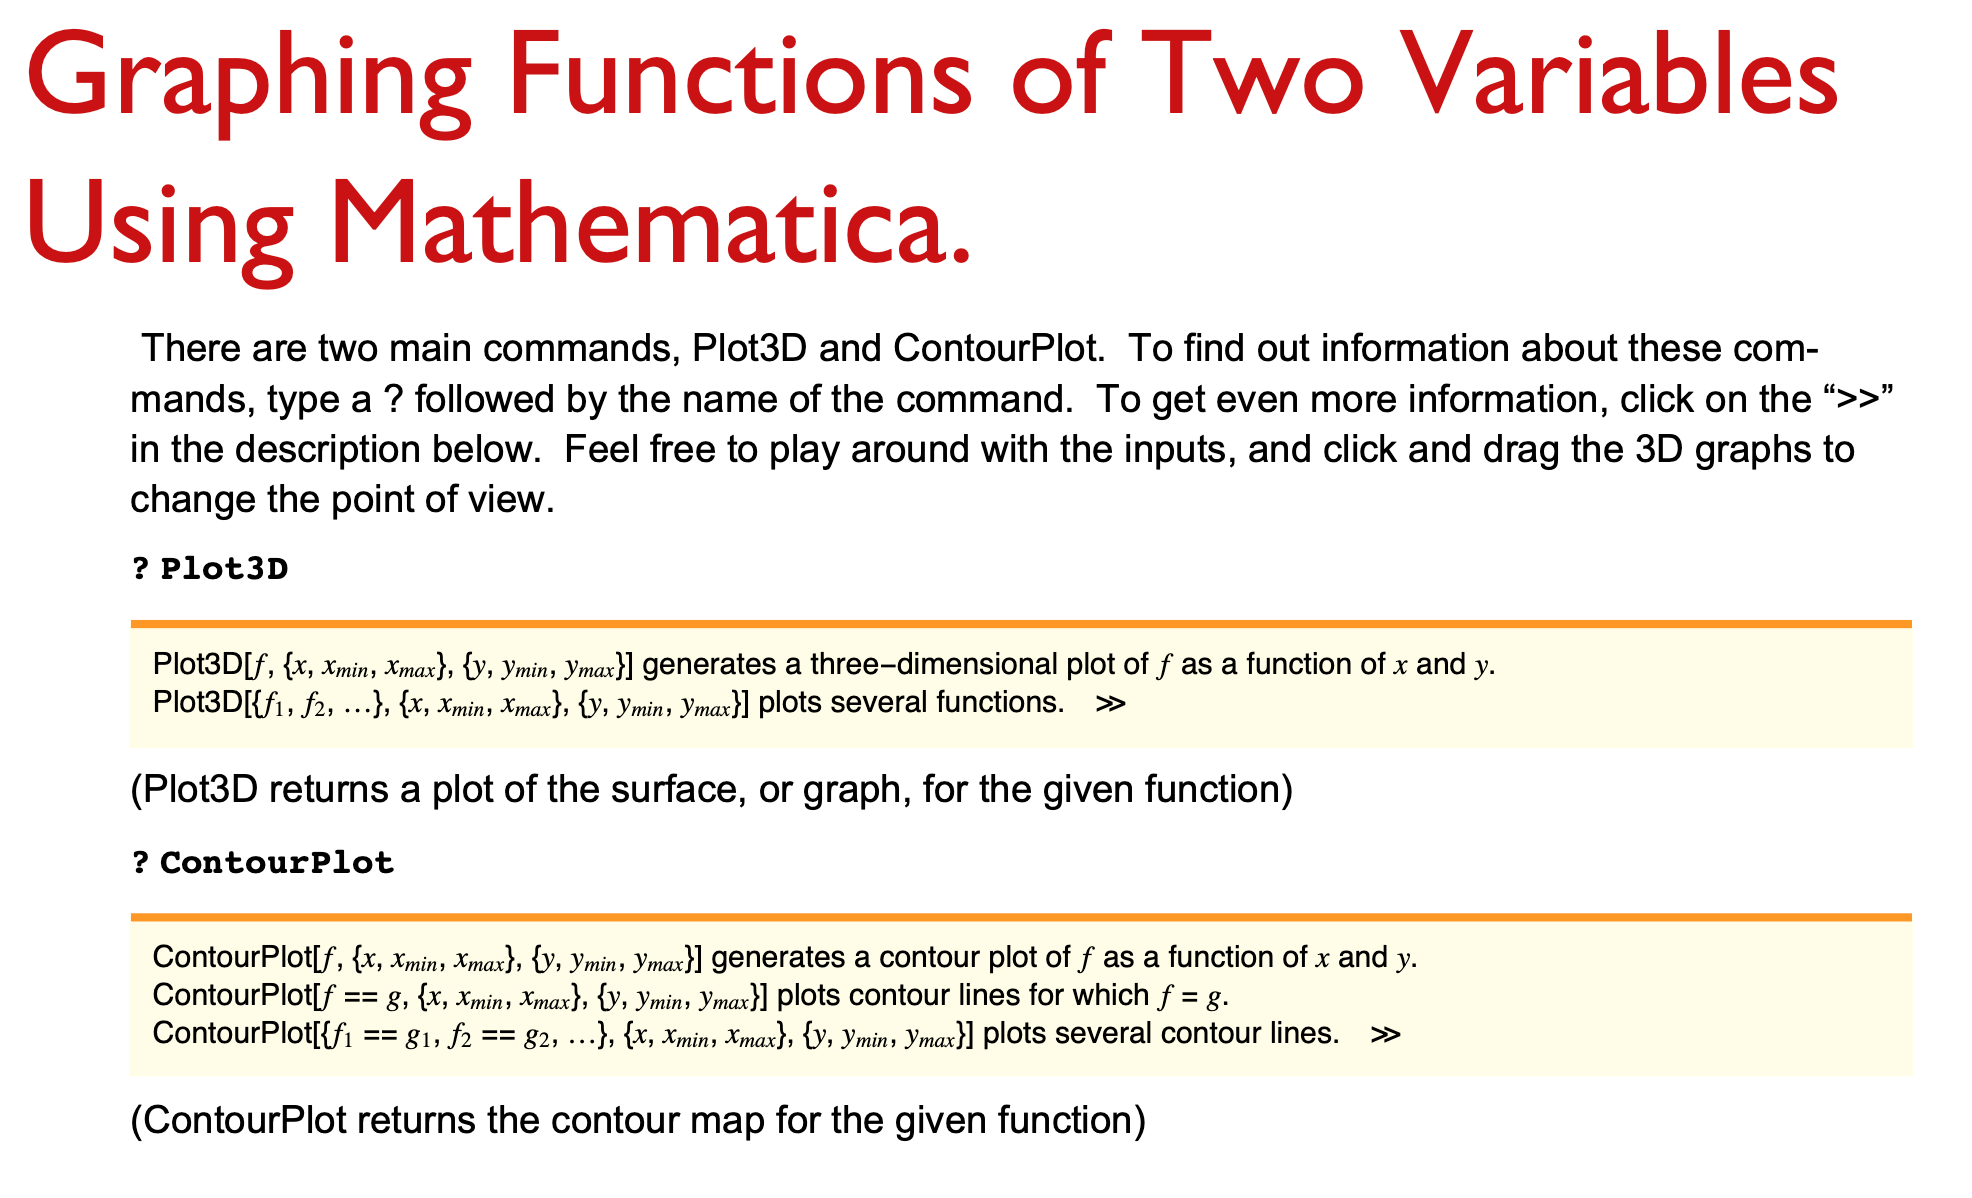
\includegraphics[width=.8\textwidth]{Mathematica-Demo1.png}

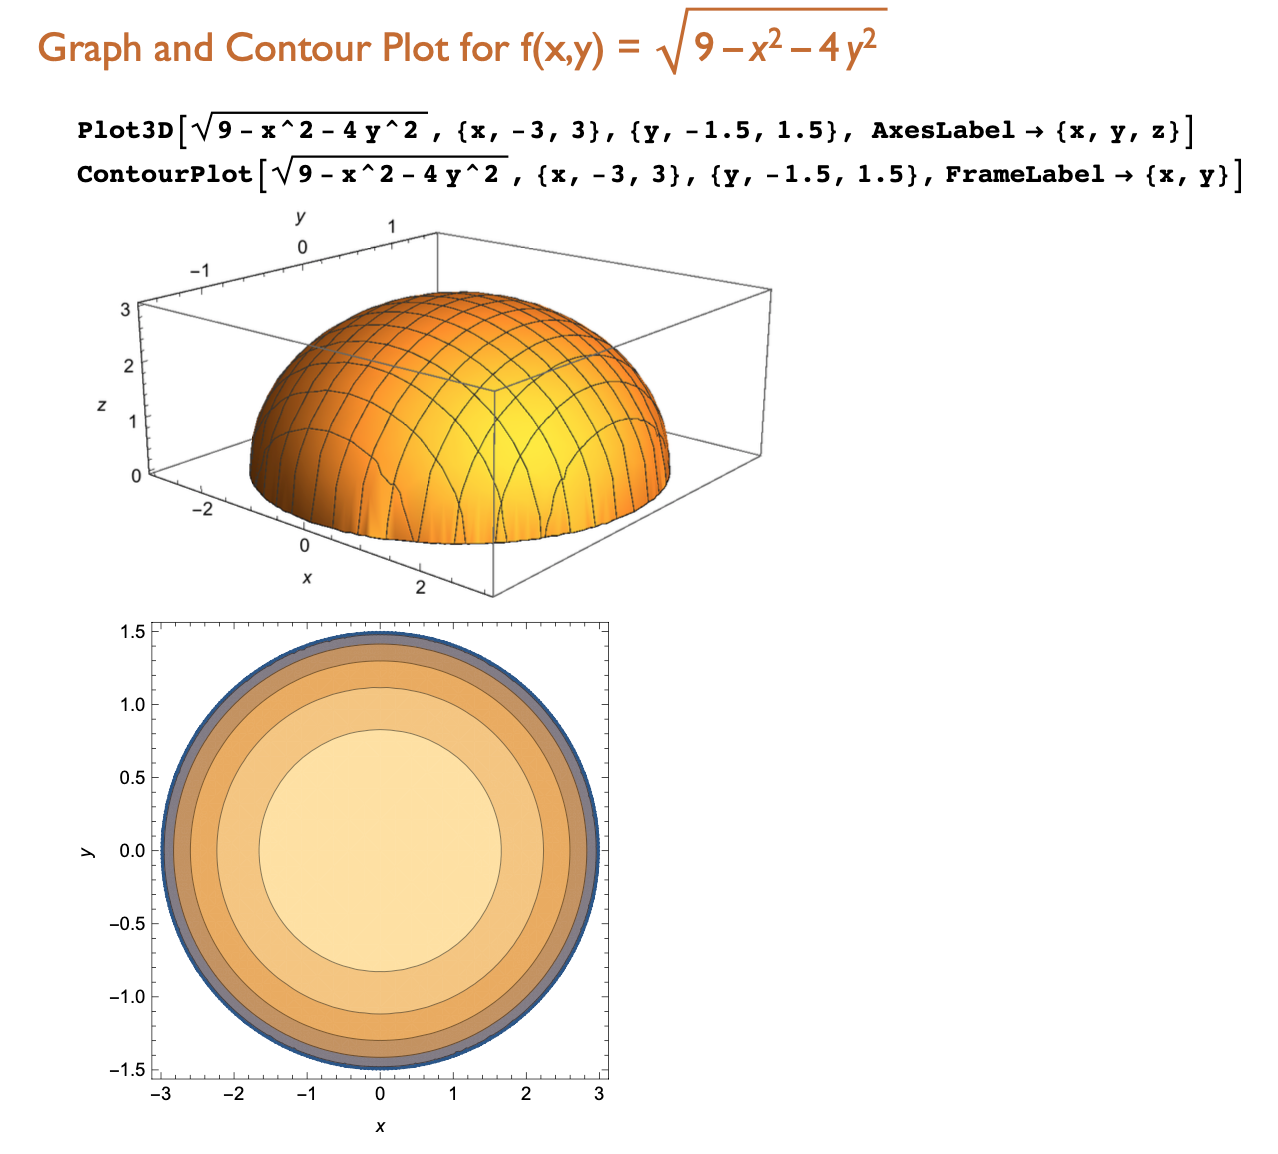
\includegraphics[width=.8\textwidth]{Mathematica-Demo2.png}
\caption{Screenshot from the Ch4s1 Mathematica Demo notebook}
\label{fig:Ch4s1demo}

\end{figure}


\section*{Section 4.1 - Group Work 2:}
(See Figure \ref{fig:dali})

\begin{figure}[!hp]
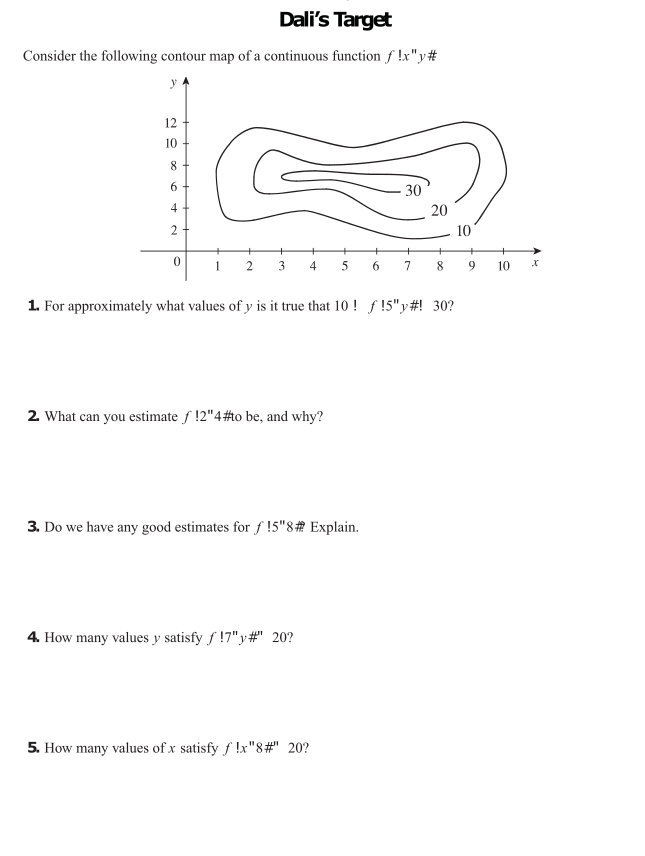
\includegraphics[]{Dalis-Target.png}
\caption{Dali's Target Group Work Activity Screenshot}
\label{fig:dali}
\end{figure}

%\pagebreak
%\vspace*{-.5in}
\section*{Section 4.2 - Limits \& Continuity:}

%\hspace*{-.8in}%\begin{minipage}{1.25\textwidth}
%\begin{framed}

\subsection*{Definitions \& Terminology:}
%\begin{multicols}{2}
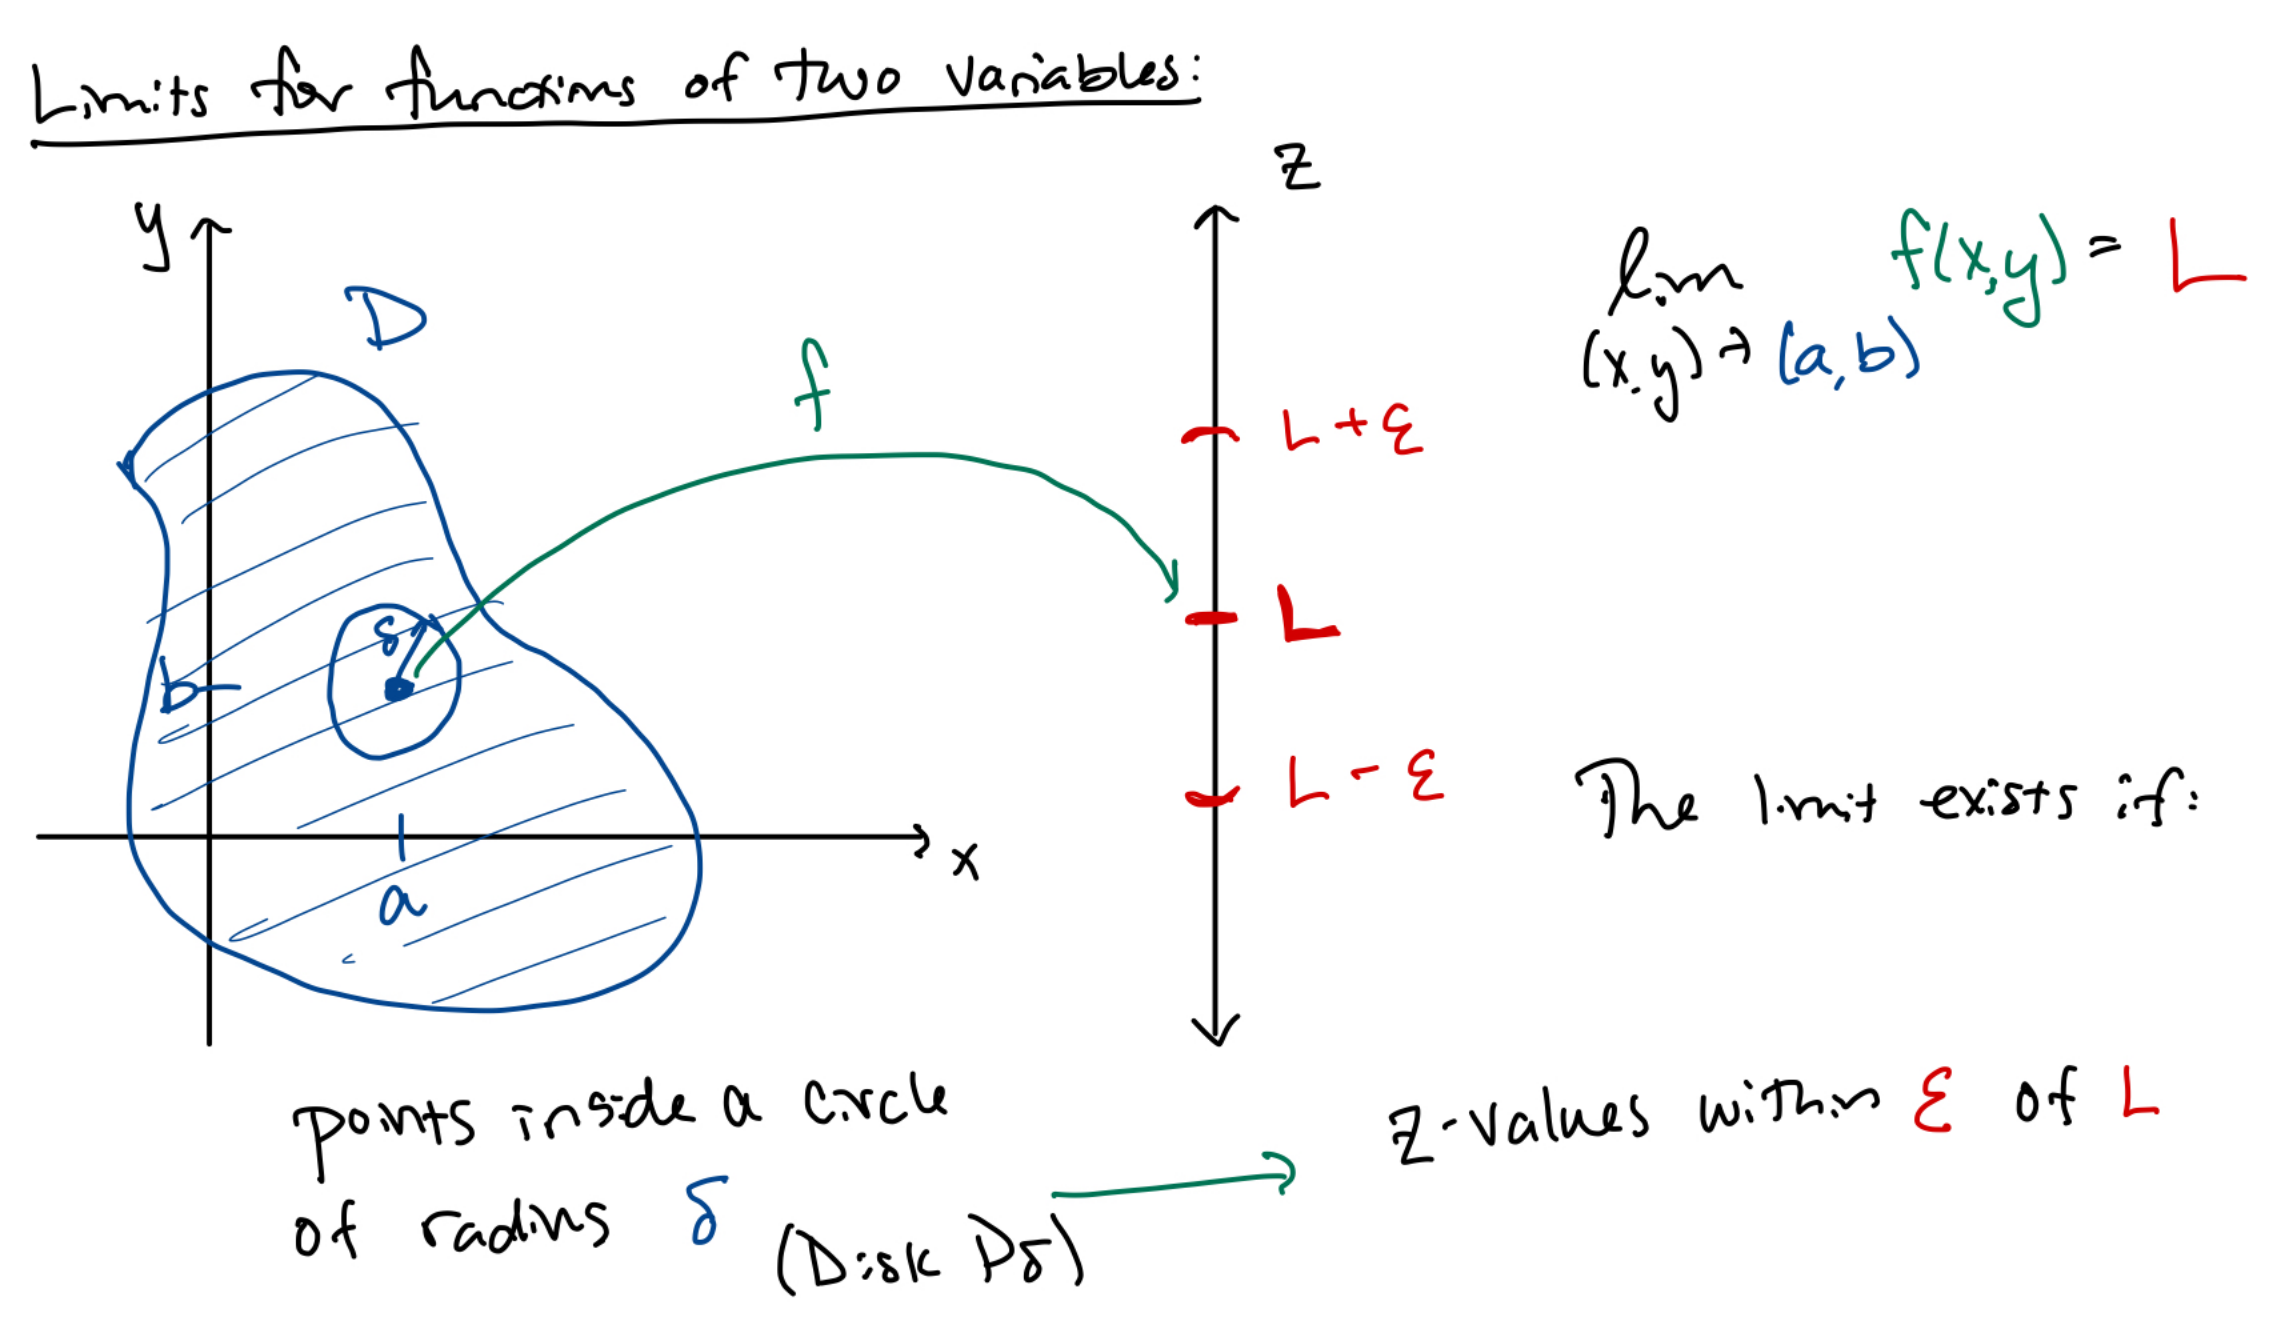
\includegraphics[]{Limit-Diagram.png}

\textbf{Formal Limit Definition:}\\
\[\lim_{(x,y)\rightarrow (a,b)} \ f(x,y) = L\]~\\

If \(\forall\  \varepsilon >0\), \(\exists\) a corresponding \(\delta >0\) such that\\~\\ if \((x,y)\ \epsilon\ D\) and \(\sqrt{(x-a)^2+(y-b)^2}<\delta\),\\~\\
 then \(\left| f(x,y)-L \right| < \epsilon\).

%\end{multicols}

\begin{itemize}

\item \textbf{WARNING: L'Hopital's Rule can only be used for expressions with a single variable.}

\item \textbf{Strategy for Evaluating Limits at the Origin:}\\
\textbf{BE SKEPTICAL!} It is easier to show that a limit does not exist than to prove that it does exist.

\begin{enumerate}
%\addtocounter{enumi}{-1}
\item Find  limits along different paths, such as:
\begin{itemize}
\item \(x-\)axis: set \(y=0\) and find the limit as \(x\rightarrow 0\)
\item \(y-\)axis: set \(x=0\) and find the limit as \(y\rightarrow 0\)
\item line of slope \(m\): set \(y=mx\) and find the limit as \(x\rightarrow 0\)
\item parabolas, etc.

\end{itemize}
If limits disagree along any two paths, or if the limit depends on the slope of the line, \(m\), the the limit does not exist.

\item If you have evidence that suggests that the limit does exist, \textbf{prove} it using one of the following methods\\
 (not covered in the text)
\begin{itemize}
\item formal \(\varepsilon-\delta\) definition of the limit %(Example 4 in text)
\item the ``Squeeze Theorem''
\item polar coordinates:\\
Set \(x=r \cos\theta\), \(y=r\sin\theta\). If the limit as \(r\rightarrow0\) exists and does not depend on the value of \(\theta\), then the limit exists.
\end{itemize}
\end{enumerate}



\item A function \(f(x,y)\) is \textbf{continuous at \((a,b)\)} if
\[\lim_{(x,y)\rightarrow (a,b)}\ f(x,y) = f(a,b).\]
We say that \(f\) is \textbf{continuous on \(D\)} if \(f\) is continuous at every point \((a,b)\) in \(D\).



\end{itemize}

%\end{framed}

%\end{minipage}


\subsection*{Examples:}

\begin{enumerate}[{Example} 1: ]
\item (Revisited) Show that the limit does not exist by showing that the limit along \(y=mx\) depends on the slope of the line.
\[\lim_{(x,y)\rightarrow (0,0)}\ \dfrac{xy}{x^2+y^2}\]

%\vfill

\item  Prove that the limit exists using: (a) the Squeeze Theorem, (b) Polar Coordinates.
\[\lim_{(x,y)\rightarrow (0,0)}\ \dfrac{xy}{\sqrt{x^2+y^2}}\]

%\vfill

\end{enumerate}

\subsection*{Mathematica Demo:}
(See Figure \ref{fig:Ch4s2demo})

\begin{figure}[!hp]
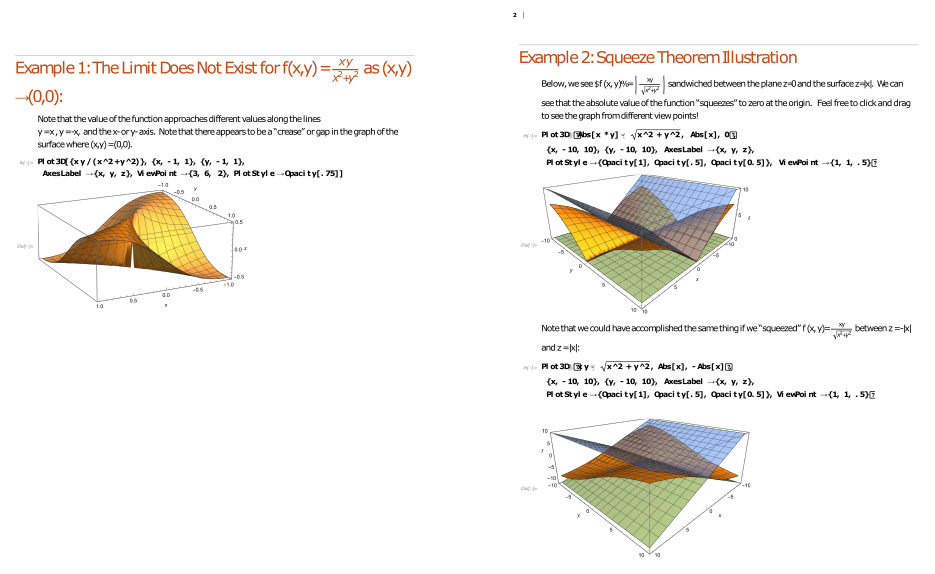
\includegraphics[]{Mathematica-Demo-Limits.png}
\caption{Screenshot from the Ch4s2 Mathematica Demo notebook}
\label{fig:Ch4s2demo}
\end{figure}

\end{document}

